\documentclass{scrartcl}
\usepackage{graphicx,tikz}
\usepackage{siunitx}
\usepackage[graphics,tightpage,active]{preview}
\PreviewEnvironment{tikzpicture}
\newlength\imagewidth
\newlength\imagescale
\begin{document}
%%%%%%%%%%%%%%%%%%%%%%%%%%
	\pgfmathsetlength{\imagewidth}{\linewidth}%
	\pgfmathsetlength{\imagescale}{\imagewidth/1563}%
	\begin{tikzpicture}[x=\imagescale,y=-\imagescale]
		\def\x{966} % scalebar-x at golden ratio of x=1563px
		\def\y{768} % scalebar-y at 90% of height of y=853px
		\node[anchor=north west, inner sep=0pt, outer sep=0pt] at (0,0) {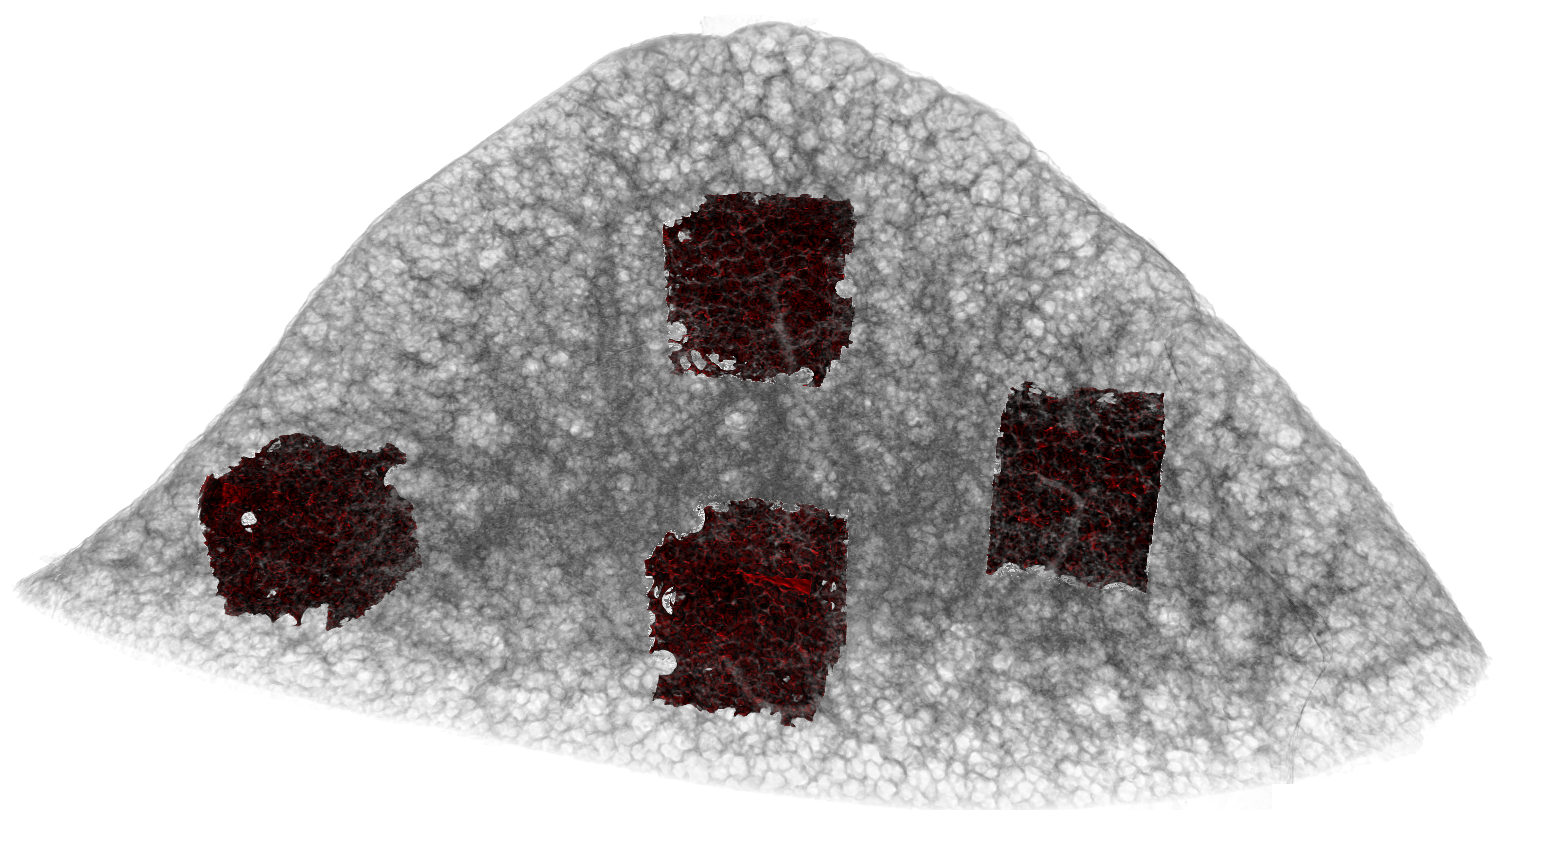
\includegraphics[width=\imagewidth]{../img/dtf-roi/ROIs-3d}};
		% 1551px = 4.0138mm > 100px = 259um > 193px = 500um, 39px = 100um
		\draw[|-|,thick] (\x,\y) -- (\x+193,\y) node [fill=white, semitransparent, midway, above] {\SI{500}{\micro\meter}};
		\draw[|-|,thick] (\x,\y) -- (\x+193,\y) node [midway, above] {\SI{500}{\micro\meter}};
		\draw ( 300,400) node [fill=white, semitransparent] {ROI 1} node {ROI 1}; % 523-497-743
		\draw ( 740,460) node [fill=white, semitransparent] {ROI 2} node {ROI 2}; % 1382-546-743
		\draw ( 760,160) node [fill=white, semitransparent] {ROI 3} node {ROI 3}; % 1324-266-289
		\draw (1080,350) node [fill=white, semitransparent] {ROI 4} node {ROI 4}; % 1863-237-604
	\end{tikzpicture}%
%%%%%%%%%%%%%%%%%%%%%%%%%%
\end{document}